\documentclass[5pt]{article}
\title{\LARGE {Note for vortex phase transition in iron-based superconductor}}
\author{\Large{Wei Cheng}}
\date{\Large{2023.3.17}}
\usepackage{amsmath,amsthm,amssymb,amsfonts, fancyhdr, color, comment, graphicx, environ}
\usepackage{verbatim}
\usepackage[UTF8]{ctex}%用于识别中文
\usepackage{underscore}%可以用来正确识别_
\usepackage{graphicx}%用于插入图片
\usepackage{geometry}
\usepackage{braket}
\usepackage{listing}
\geometry{a4paper,scale=0.85}
\usepackage{hyperref}%用于插入链接
\hypersetup{
	colorlinks=true,
	linkcolor=blue,
	filecolor=magenta,      
	urlcolor=blue,
}%插入链接的性质
\usepackage{pythontex}
\usepackage{import}
\usepackage{subfiles}
\usepackage{xifthen}
\usepackage{pdfpages}
\usepackage{transparent}
\usepackage{framed}
\usepackage{tcolorbox}
\usepackage[dvipsnames,svgnames]{xcolor}
\usepackage{abstract}
\usepackage{pgfplots,tikz}
\tcbuselibrary{skins,breakable,xparse}
\usepackage{shadowtext}
\usepackage{titlesec}
\usepackage{titletoc}
\usepackage{setspace}
\usepackage{float}
\usepackage{enumitem}  
\usepackage[normalem]{ulem}
\usepackage[charter]{mathdesign}
\usepackage{shadowtext}
\usepackage{setspace}
\usepackage{tabularcalc}
\usepackage{booktabs}




\renewcommand{\abstractname}{\Large Abstract}
\definecolor{mygreen}{rgb}{0.8,1,0.73}
\definecolor{linegreencolor}{rgb}{0,0.4,0}
\definecolor{myblue}{rgb}{0.22,0.73,0.91}
\definecolor{LightBlue1}{rgb}{0.22,0.73,0.91}
\definecolor{myteal}{cmyk}{0.5,0,0.15,0}
\definecolor{myred}{RGB}{255,182,185}
\definecolor{myredline}{RGB}{228,44,100}

\titleformat*{\section}{\Large\bfseries\filcenter}
\titleformat*{\subsection}{\Large\bfseries}
\titleformat*{\subsubsection}{\Large\bfseries}
\titleformat*{\paragraph}{\large\bfseries}
\titleformat*{\subparagraph}{\large\bfseries}

\renewcommand*\contentsname{\hfill \LARGE{Content} \hfill}


\begin{document}
	\maketitle
	\Large
	\tableofcontents
	\everymath{\displaystyle}
	\begin{abstract}
		\Large
		Iron-based superconductor is a very good platform to search Majorana zero model due to it's topological band and high temperature superconductor.Here we search the vortex phase transition in iron-based superconductor.First we can use the $k\cdot p$ method to construct the Hamiliton.Then use the Hamiliton we can do some numerical calculation and theory analysis.
	\end{abstract}
\section{$k\cdot p$ construct Hamiliton}
The space group of iron-based superconductor is P4/nmm,it include the frational translate,so it can't can be seen the the direct product of the translate group and the point group.But along the $\Gamma-Z$,it can be seen the $D4h$ group。At the same time,we can know the band near the fermi surface of the iron-based superconductor are $p_z,d_{xz},d_{yz}$ orbit.So we can choose the basics $\ket{p_z,\uparrow},\ket{p_z,\downarrow},\ket{d_{xz+iyz},\downarrow},\\
\ket{d_{xz-iyz},\uparrow},\ket{d_{xz+iyz},\uparrow},\ket{d_{xz-iyz},\downarrow}$ to construct our Hamiliton.For any $6\cdot 6$matrix,we can break down to the linear superposition of 36 basics matrix.
\begin{align}
	H(\vec{k})=\sum_{ij}f_{ij}(\vec{k})M_{ij}
\end{align}
we can construct the 36 basics Hermitian matrix from the direct product of the Pauli matrix and the Gellman matrix.
\begin{align}
	M_{ij}=G_i\otimes \sigma_j
\end{align}
The $G_i$ means the Gell-Man matrix,it's range is from 0 to 8.The $\sigma_j$ means the Pauli matrix,it's range is from 0 to 3. 
At the same time,because we need to consider the spin orbit coupling,so we neend sonsider the double group,we can find the character table of the D4h.
\begin{figure}[H]
	\centering
	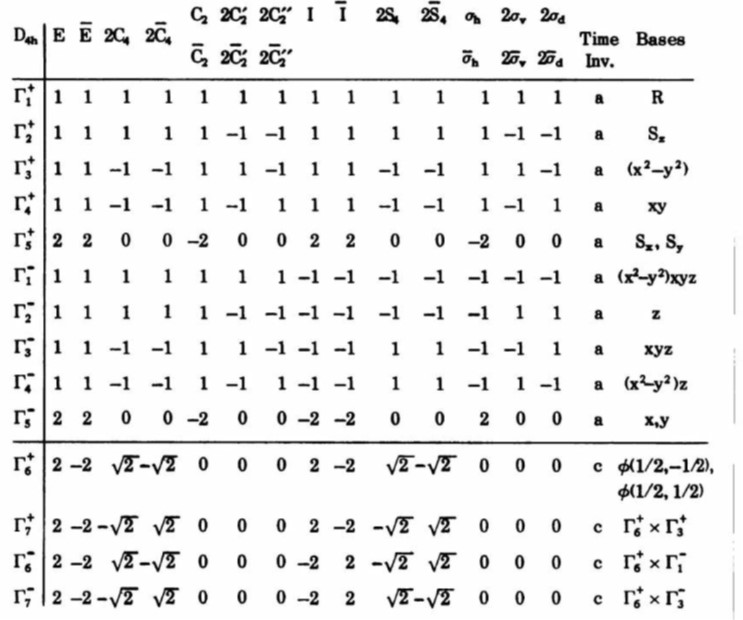
\includegraphics[scale=0.8]{figure/1}
	\caption{}
	\label{}
\end{figure}
We can get the generator of D4h group is $C_{4z},C_{2x}^{'},Inversion$.At the same time,the system has the time reversal symmetry.We can get the transformation matrix in the basics before we mentioned.
\begin{normalsize}
\begin{align}
	C_{4z}=
	\frac{1}{\sqrt{2}}
	\begin{pmatrix}
		1-i&&&&&\\
		&1+i&&&&\\
		&&1-i&&&\\
		&&&1+i&&\\
		&&&&-1-i&\\
		&&&&&-1+i
	\end{pmatrix}
\qquad
C_{2x}=\begin{pmatrix}
	&i&&&&\\
	i&&&&&\\
	&&&i&&\\
	&&i&&&\\
	&&&&&i\\
	&&&&i&
\end{pmatrix}
\end{align}
\begin{align}
	I=\begin{pmatrix}
		-1&&&&&\\
		&-1&&&&\\
		&&1&&&\\
		&&&1&&\\
		&&&&1&\\
		&&&&&1
	\end{pmatrix}
\qquad
T=
\begin{pmatrix}
&-1&&&&\\
1&&&&&\\
&&&-1&&\\
&&1&&&\\
&&&&&-1\\
&&&&1&\\	
\end{pmatrix}
\mathcal{K}
\end{align}
\end{normalsize}
we can get the character table of the polynomials
of the momentum k
\begin{align}
	\nonumber
	\begin{tabular}{ccc}
		\toprule
		\midrule
		k polynomial & representation & time reversal \\
		1,$k_x^2+k_y^2$,$k_z^2$ &$\Gamma_1^{+}$&+\\
		$k_xk_y$&$\Gamma_4^{+}$&+\\
		$k_x^2-k_y^2$&$\Gamma_3^{+}$&+\\
		$\{k_xk_z,k_yk_z\}$&$\Gamma_5^{+}$&+\\
		$\{k_x,k_y\}$&$\Gamma_5^{-}$&-\\
		$k_z$&$\Gamma_2^{-}$&-
	\end{tabular}
\end{align}
we can get the character table of $M_{ij}$,Then we can mul

\begin{figure}[H]
	\centering
	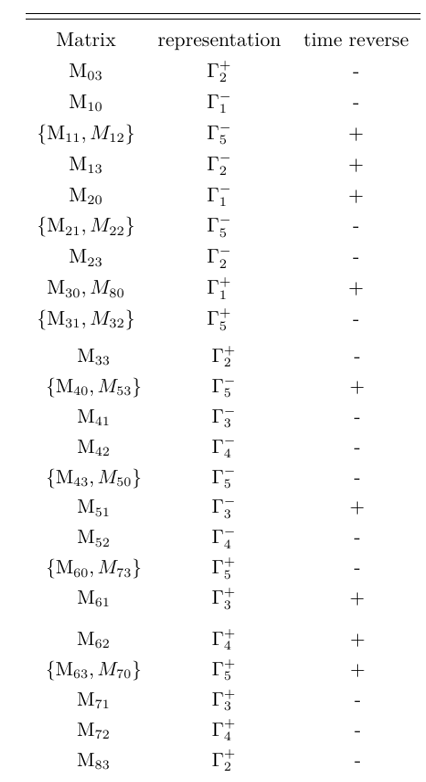
\includegraphics[scale=0.8]{figure/2}
	\caption{}
	\label{}
\end{figure}




\section{Vortex Phase Transition}





\end{document}